

\chapter{\selfour Basics}
\label{chap:sel4}

So far we have provided a general background on real-time scheduling and resource sharing.
As the final piece of background we now present an overview of the concepts relevant to the temporal behaviour of our implementation platform, \selfour.

\selfour is a microkernel that is particularly suited to safety-critical, real-time systems with one
major caveat: time is not treated as a first class resource, leading to deficiency in real-time scheduling support. 
Three main features of \selfour support this claim: it has been formally verified for correctness~\citep{Klein_EHACDEEKNSTW_09} and other properties~\citep{Sewell_WGMAK_11}; All memory management, including kernel memory, is all at user-level~\citep{Elkaduwe_Derrin_06}; Finally it is the only \gls{OS} to date with full \gls{WCET} analysis~\citep{Blackham_SCRH_11}.
The scheduler in \selfour has been left intentionally underspecified~\citep{Petters_EH_12} for later work and as a result has a very informal notion of time.
The current implementation is a placeholder, and follows the traditional L4 scheduling model~\citep{Ruocco_06} --- a fixed-priority, round-robin scheduler with 256 priorities.

In this section we will present the current state of relevant \selfour features in order to highlight deficiencies and motivate our changes.
We will outline the existing scheduler, the API curiosity that is \yield, and how \gls{IPC} interacts with scheduling, followed by an analysis of how the current mechanisms can be used in real-time systems.


First we introduce the basics of \selfour: kernel memory management, capabilities, \gls{IPC} and
signalling. \Cref{f:legend-1} shows the legend for diagrams in this section. 

\begin{figure}
    \centering
    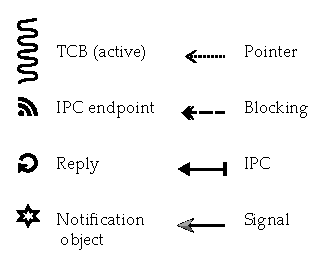
\includegraphics[width=0.5\textwidth]{legend-1}
    \caption{Legend for diagrams in this section}
    \label{f:legend-1}
\end{figure}

\section{Capabilities}
\label{s:capabilities}

As a capability-based \gls{OS}, access to any resource in \selfour is via capabilities (recall
\Cref{s:os-capabilities}). Capabilities to all system resources are passed to the initial task---the first
user-level thread started in the system---which can then allocate resources as appropriate.
Capabilities exist in a \emph{capability space} that can be configured per thread or shared between
threads. 

Capability spaces (\code{cspace}s) are analogous to address spaces for virtual memory: where address spaces map
virtual addresses to physical addresses, capability spaces map object identifiers to access rights.
Cspaces are formed of \emph{capability nodes} \code{cnode}s which contain capabilities, analogous to page tables
in virtual memory, and can contain capabilities to further \code{cnode}s, which allows for multi-level
cspace structure. A cspace address refers
to an individual entry in some CNode in the capability space, and may be empty or contain a
capability to a specific kernel resource. For brevity, a cspace address is referred to as
a slot. 

% access rights
Each capability has three potential access rights: read, right and grant. How those rights affect
the resource the capability provides access to depends on the type of resource, and is explained in
the next section.

% badges and operations
Various operations can be done on capabilities, which are summarised in \cref{t:capability_ops}.
When a capability is copied or minted, it is said to be \emph{derived} from the original capability.
All derived capabilities can be deleted by using \code{revoke}.
There are restrictions on which capabilities can be derived and under what conditions, depending on
what the capability provides access to. 
\emph{Badging} is a special type of derivation which allows specific capability types to be copied
with an unforgeable identifier. We discuss derivation restrictions and the use of badges further
in this chapter.
Any individual capability can be deleted, or revoked. The former simply removes a specific
capability from a capability space, the latter removes all child capabilities.

\begin{table}
    \centering
    \rowcolors{2}{gray!25}{}
    \begin{tabular}{l p{0.8\textwidth}}\toprule
    \emph{Operation}    & \emph{Description}\\\midrule
    \code{Copy}         & Create a new capability in a specified CNode slot, which is an exact copy
                         of the other capability and refers to the same resource. \\
    \code{Mint}         & Like copy, except the new capability may have diminished rights and/or be
                          badged. \\
    \code{Move}         & Move a capability from one slot to another slot, leaving the previous slot
                          empty. \\
    \code{Mutate}       & Like move, except the new capability may have diminished rights and/or be
                          badged. \\
    \code{Rotate}        & Atomically move two capabilities between three specified slots. \\
    \code{Delete}        & Remove a capability from a slot. \\
    \code{Revoke}        & Delete any capabilities derived from this capability. \\
    \code{SaveCaller}    & Saves the kernel generated resume capability into the designated slot. \\
    \bottomrule 
    \end{tabular}
    \caption{Summary of operations on capabilities provided by baseline \selfour~\citep{seL417}}.
     \label{t:capability_ops}
\end{table}

\section{System calls and invocations}

\selfour has a two-level system call structure, based on capabilities. The first level of system calls
are distinguishable by system call number, as listed in \cref{t:system-calls}. The majority of
system calls are for communication; \code{send}, \code{nbsend}, \code{call}, \code{reply} are for
sending messages; \code{recv}, \code{nbrecv} for receiving messages; and \code{yield} for
interacting with the scheduler.

The second level of system calls are called \emph{invocations} and are modelled as sending a message
to the kernel. All invocations are conducted by a sending system call. The kernel is modelled as if
it is waiting for a message and receives one every time a system call is made. 
To determine the operation, the rest of the arguments to an invocation are encoded as a message to
the kernel. Each capability type has a different set of invocations available, and on a send to the
kernel the capability is decoded to determine the action the kernel should take. 

\begin{table} 
    \centering
    \rowcolors{2}{gray!25}{}
    \begin{tabular}{l}\toprule
        \emph{System call} \\\midrule
        \texttt{send} 
        \texttt{nbsend}    \\
        \texttt{call}      \\
        \texttt{recv}      \\
        \texttt{nbrecv}    \\
        \texttt{reply}     \\
        \texttt{replyrecv} \\
        \texttt{yield}     \\
        \bottomrule
    \end{tabular}
    \caption{\selfour system call summary.}
    \label{t:system-calls}
\end{table}

All of the operations on capabilities are that are listed in \cref{t:capability_ops} are invocations
on \code{cnode} capability addresses. For example, to copy a capability, one uses \code{call} on a
\code{cnode}, and provides the invocation code for copy, as well as the arguments. In the case of
copy, one provides the slot of the capability being copied, in addition to the destination
\code{cnode} and
slot. 

\section{Kernel Resources}

Capabilities provide access to specific kernel resources, a brief summary of which is shown in
\cref{t:kernel_objects}. 


% table of object types 
\begin{table}
    \centering
    \rowcolors{2}{gray!25}{}
    \begin{tabular}{l p{0.6\textwidth}}\toprule
    \emph{Object}    & \emph{Description}\\\midrule
    CNode            & A fixed size table of capabilities. \\
    \Gls{TCB}        & A thread of execution in \selfour.\\
    Endpoint  & Ports which facilitate \gls{IPC}. \\
    Notification object & Arrays of binary semaphores.\\
    Vspace     & Top level paging structure. \\
    PageTable  & Page table structures and address space IDs.\\
    Page       & Mappable physical memory. \\
    Interrupt & Allow access to specific hardware interrupts.\\
    Untyped    & Memory that can be retyped into other types of memory, including untyped.\\
    \bottomrule
    \end{tabular}
    \caption{Major object types in \selfour, excluding platform specific objects. For further detail
    consult the \selfour manual~\citep{seL417}}.
     \label{t:kernel_objects}
\end{table}

All kernel memory in \selfour is managed at user-level and accessed via capabilities
which is key to \selfour's isolation and security, but also essential for
understanding the complexity of kernel design. Additionally, this allows for the ultimate in policy
freedom: all resource allocation is done from user-level by those holding the appropriate
capabilities.

In the initial system state, capabilities to all resources are given to the first task started by
the system, the \emph{root task}. Then according to system policy the root task can divide up and
delegate system resources.  This includes capabilities to all memory, apart from the small section
of static memory used by the kernel. The kernel itself has a large, static \emph{kernel window}
initialised at boot time, which
consists of memory mapped such that it is directly writeable by the kernel. The kernel window size
is platform specific, but is 500MiB on all 32-bit platforms.  

\subsection{Untyped}

All memory starts as \emph{untyped} memory, and capabilities to all available untyped memory are placed in the
cspace of the root task on boot. Each untyped consists of a start address, a size, and a flag
indicating whether the untyped is writeable by the kernel or not. Memory reserved for devices and
memory outside the kernel window is not readable or writeable by the kernel. 

Untyped objects have only one invocation: \emph{retype}, which allows for large untyped objects to
split into smaller objects of a different size and type, including frames, page tables, cnodes, etc. 
While the majority of objects in \selfour have a platform-dependent size fixed at compile time, some
are sized dynamically at runtime, \eg untyped and CNodes, which can be any power of two size.

Any capability to memory---untyped or not---is a capability to a specific object in memory,
containing a pointer to that object. When retype is used to create sub-objects in an untyped, those
subsets of memory will not become available for retyping again until every capability to that object has been deleted, somewhat like reference counting pointers.

\subsection{Control capabilities}

Not all capabilities refer to memory-based resources, such as interrupts and \IO ports.
In order to obtain capabilities to specific interrupts or ranges of \IO ports, the root task is
provided with non-derivable control capabilities which can be invoked to place specific hardware
resource capabilities in empty \code{cslot}s.


% control caps, normal caps
% operations


\subsection{Untyped}

Object capabilities are 
object is deleted will the object itself be deleted. Object capabilities contain a pointer to the
actual kernel object. 



All memory in \selfour starts as \emph{untyped} memory, capabilities to which is granted to the
initial task in the system as part of the boot process. The initial task can then create all
types of memory, including further untyped, with an operation known as \emph{retyping}. As a result,
any object with a pointer to another object must have a back pointer to update should that object be
deleted, in order to avoid stray pointers in the kernel. 


\subsection{Thread control blocks}

\Glspl{TCB} represent an execution context and manage processor time in \selfour. Each \gls{TCB} is
associated with a cspace and a top level virtual memory object, specified by capabilities, which may
be shared with other threads. 
Additionally threads have an IPC buffer, which is a page shared between the kernel and the thread
for messages. 
Threads have a timeslice attribute, which specifies the amount of milliseconds until that thread is
preempted, and a priority for the fixed priority scheduler.

% table of tcb invocations
\begin{table}
    \centering
    \rowcolors{2}{gray!25}{}
    \begin{tabular}{l p{0.8\textwidth}}\toprule
    \emph{Operation}    & \emph{Description}\\\midrule
        \code{Resume}               & Place a thread in the scheduler.\\ 
        \code{Suspend}              & Remove a thread from the scheduler.\\
        \code{WriteRegisters}       & Configure a threads execution context.\\
        \code{ReadRegisters}        & Read a threads execution context.\\
        \code{SetAffinity}          & Set the CPU on which this thread should run.\\
        \code{SetIPCBuffer}         & Set the page to use for the IPC buffer.\\
        \code{SetPriority}          & Set the priority of this TCB.\\
        \code{BindNotification}     & TODO \\
    \bottomrule 
    \end{tabular}
    \caption{Summary of operations on TCBs. Further operations are available that batch several
    setters to reduce thread configuration overheads.}.
     \label{t:tcb_ops}
\end{table}


\subsection{Endpoints}
\label{s:endpoints}

In the \selfour model,
\gls{IPC} takes place via endpoints, which represent a general communication port. Any thread with a
capability to an endpoint can send and receive messages on that endpoint, subject to the access
rights. Most messages sent fit into registers, however messages exceeding this platform-dependent
size are stored in the \gls{IPC} buffer, a kernel-writeable frame per
thread. 

IPC can be one-way, where the sender blocks until the message is sent then may continue
(\texttt{send()}) , or two-way,
where the sender blocks until a reply message is sent (\texttt{call()}). One-way IPC may also be
non-blocking, where the message is only sent if a receiver is already present.
Multiple senders and receivers can use the same endpoint, and which act as \gls{FIFO}
queues. 

\begin{figure}
    \centering
    \begin{subfigure}[h]{0.48\textwidth}
        \centering
        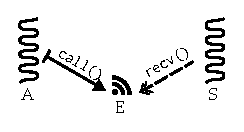
\includegraphics[width=\textwidth]{ipc1}
        \caption{Phase 1}
        \label{f:ipc1}
    \end{subfigure}%
    \begin{subfigure}[h]{0.48\textwidth}
        \centering
        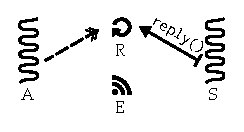
\includegraphics[width=\textwidth]{ipc2}
        \caption{Phase 2}
        \label{f:ipc2}
    \end{subfigure}
    \caption{IPC phases: (a) shows the initial IPC rendezvous, (b) shows the
    reply phase. See \Cref{f:legend-1} for the legend.}
    \label{f:ipc}
\end{figure}

Two-way IPC has two phases, as \cref{f:ipc} illustrates: rendezvous and reply.

\Cref{f:ipc1} demonstrates the rendezvous phase, where regardless of the order of operations, 
when one thread blocks (\code{recv()}) on the endpoint and another thread sends on that endpoint
then a message is sent. This occurs for both one-way and two-way \gls{IPC}.

The reply phase, illustrated in \Cref{f:ipc2}, only occurs if the sender used \texttt{call} to send
the \gls{IPC}. In this case, a one-off \emph{resume} capability is generated, which the caller ($A$)
blocks on, and the receiver ($S$) sends a reply message to, waking the caller. Receivers can save
the \emph{resume} capability to send a reply to later, but otherwise the resume capability is
installed in the \gls{TCB} CNode. The \emph{reply} system call directly invokes the resume
capability in this slot. 

% fastpath
Given \gls{IPC} performance is critical to overall system performance in a microkernel, \selfour
contains two \gls{IPC} fastpaths which is used when the following, common-case conditions are satisfied:

\begin{enumerate}
    \item the sender is using \texttt{call()} or the receiver is using \texttt{replyrecv()},
    \item there are no threads of higher priority than the thread being woken in the scheduler,
    \item the thread to be switch to has a valid address space and has not faulted,
    \item and the message fits in registers.
\end{enumerate}

Endpoint capabilities can be minted with unique, unforgeable badges which are delivered to the
receiver with the rest of the IPC message. This provides a mechanism for identifying senders.

\subsection{Fault handling}

\glspl{TCB} can have a specific fault endpoint registered, on which the kernel can send simulated
\gls{IPC} messages containing information about the fault. Fault handling threads can block on this 
endpoint. When a fault message is delivered to the fault endpoint, the kernel blocks the faulting
thread. The fault handling thread can then reply to this message to resume the thread and reset its
registers. If no fault endpoint is present, the
thread is rendered inactive and no fault message is sent. 

\subsection{Notifications}

\TODO{A diagram of the notification word}
Notification objects are an array of binary semaphores used to facilitate asynchronous communication in \selfour, either from other threads via \texttt{send()} or from
interrupts.  The signals are non-blocking, as the badge of the notification capability is simply
bitwise ORed with a data word stored in the notification object itself. When a receiver blocks on a
notification object (\texttt{recv()}), if the badge has already been set it the receiver will
receive it immediately, otherwise the receiver will block immediately. Receivers can also poll a
notification object with \texttt{nbrecv()}.

% notifications, interrupts, aep-binding
\begin{figure}
    \centering
    \begin{subfigure}[h]{0.48\textwidth}
        \centering
        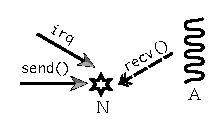
\includegraphics[width=\textwidth]{signal1}
        \caption{Notification}
        \label{f:signal1}
    \end{subfigure}%
    \begin{subfigure}[h]{0.48\textwidth}
        \centering
        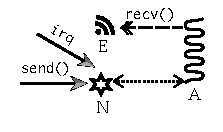
\includegraphics[width=\textwidth]{signal2}
        \caption{Bound notification}
        \label{f:signal2}
    \end{subfigure}
    \label{f:signal}
    \caption{Signals via a notification object. See \Cref{f:legend-1} for the legend.}
\end{figure}


\Cref{f:signal1} shows signal handling, where a thread A receives a signal and an interrupt at the
same time. In this case, the interrupt handler has a badged capability to the notification object,
$N$, as does the signaller. Both badges will be combined with a bitwise OR and delivered to the
receiver.

Signals can also be received by threads waiting on \gls{IPC}, as shown in \Cref{f:signal2}. A
\gls{TCB} object is bound to a notification object, establishing a link between them. Badges can be
used to determine whether a message was received from the endpoint or a signal on the notification object.

\subsection{System calls}

Over the last few sections we have indirectly presented several system calls for \gls{IPC} and
signalling. \Cref{t:system-calls} shows all the system calls available in \selfour. Communication
with the kernel itself is modelled as \gls{IPC} by using \texttt{call()} on kernel object
capabilities. Each capability has a set of \emph{invocations} which allow for methods on that object
to be used \eg binding a \gls{TCB} and notification object.

\subsection{Thread states}

As depicted in \Cref{f:thread_state}, threads in \selfour can be inactive, running or blocked on a
specific object. The thread state encodes the object which the thread is blocked on. 

\begin{figure}[h!tb]
    \centering
    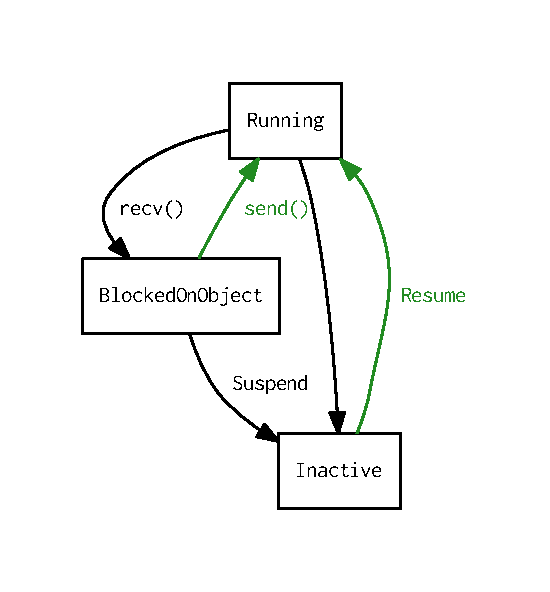
\includegraphics[width=1.1\textwidth]{thread_state}
    \caption{Thread state transitions in \selfour}
    \label{f:thread_state}
\end{figure}


\section{Scheduler}

The scheduler in \selfour is priority-based round-robin with 256 priorities (0 --- 255), implemented as an array of lists: one list of ready threads for each priority level. 
At a scheduling decision, the kernel chooses the head of the highest-priority, non-empty list, and
removes it from the relevant scheduler queue, which is referred to as \emph{Benno Scheduling}, named
after its original author.
The kernel previously used \emph{lazy scheduling}, leaving the current thread in its run queue, however this was replaced in favour of Benno scheduling to reduce the WCET of the kernel. 

Scheduling decision complexity is $O(1)$ as a two-level bit field tracks the highest priority with a runnable thread.

Kernel time is accounted for in ticks, with a static tick length defined at compile time (CONFIG\_TIMER\_TICK\_MS).
Threads have a timeslice field which represents the number of ticks they are eligible to run. 
This value is decremented every time a timer tick is handled, and when the timeslice is exhausted the thread is appended to the relevant scheduler queue, with a replenished timeslice.
The reload value of the timeslice is also defined at compile time (CONFIG\_TIME\_SLICE).

In an unrealistically simple system, where threads run at the same priority and do not communicate, it is possible to analyse temporal behavior on \selfour: threads will run for the timeslice value in round-robin order.
However, the allocation of ticks to threads is not actually that simple due to yield behaviour, preemption and \gls{IPC}. 

\subsection{Priorities}

Like any priority-based kernel without temporal isolation mechanisms, time is only guaranteed to the highest priority threads.
Priorities in \selfour act as informal capabilities: threads cannot create threads at priorities higher than their current priority, but can create threads at the same or lower priorities.
If threads at higher priority levels never block, lower priority threads in the system will not run.
As a result, a single thread running at the highest priority has access to 100\% of processing time.
However, even this becomes unclear once there is more than one thread at a priority: if two threads are running, they can both access 50\% of processing time.
If one of two threads blocks, the other gets 100\% of processing time and vice versa.
There is no way to enforce a certain processor allocation and how CPU time a thread receives is up
to priorities and the behaviour of other threads in the system, which is impossible to guarantee.

\subsection{Accounting}
% I think this should move to the design section?
\selfour has a tick-based scheduler, where ticks are accounted to the currently running thread,
meaning that temporal isolation in servers is not possible and accuracy is traded for precision, as
discussed in \Cref{s:tick-v-tickless}.

Similarly, the \texttt{yield} system call will not alter the timeslice of the current thread, and
only donates a portion of the current tick to the next thread in the round-robin scheduler. 

\subsection{Domain scheduler}

A recent addition to the \selfour kernel adds the ability to guarantee complete temporal isolation and deterministic scheduling between sets of threads, using the concept of scheduling \emph{domains}.
Threads are assigned to domains, each of which has a separate array of lists of threads over the priority range.
Each domain runs for a fixed amount of ticks, and domains are scheduled sequentially and deterministically.
Cross-domain \gls{IPC} is delayed until a domain switch, and \texttt{yield} between domains is not
possible. When there there are no threads to run while a domain is scheduled, a domain-specific idle thread will run until a switch occurs.

The domain scheduler can be leveraged to achieve temporal isolation however since domains cannot be
preempted, it is only useful for cyclic, non-preemptive scheduling with scheduling order and
parameters computed-offline.
In such a scenario each real-time task could be mapped to its own domain, and each task would run for its specified time before the domain scheduler switched to the next thread.
Any unused time in a domain would be wasted, and spent in the idle thread.

Such a scheduler is only suitable for closed systems and results in low system utilisation.
Dynamic real-time applications with shared resources and high system utilisation are not compatible
with the domain scheduler, as they require preemption.

\section{RT support}

We introduced basic \selfour concepts and terminology, and investigated mechanisms that effect
timing behaviour in the kernel: the scheduler, priorities, yield and IPC. 
In this section we will look at how real-time scheduling could be implemented with those mechanisms.

There are several options for implementing a real-time scheduler in the current version of \selfour: leveraging the domain scheduler, using the priority scheduler or implementing a scheduling component to run at user-level. 
The domain scheduler offers low utilisation for strictly closed
systems with strict temporal partitioning and no preemption, so is clearly insufficient, as
discussed in \Cref{sec:rt-scheduling}.

The priority scheduler could be leveraged to implement a rate-monotonic scheduler.
However, this requires complete trust in every thread in the system, as there is no mechanism for temporal isolation: if one thread executes for too long, other threads will miss their deadlines.
Essentially the only thread with a guaranteed CPU allocation is the highest priority thread, which under rate-monotonic priority assignment is not the most critical thread in the system, but the thread with the highest rate.
Additionally, periodic threads driven by timer interrupts rather than events would need to share a user-level timer.

\begin{table}
	\centering
	\begin{tabular}{lp{2cm}p{2cm}p{2cm}p{2cm}} \toprule
        & \emph{Temporal isolation} & \emph{Utilisation} & \emph{Low kernel overheads} &
        \emph{Dynamic}\\
        \midrule
Domain scheduler          & \yes               & \no         & \yes        & \no    \\
Priority scheduler        & \no                & \yes        & \yes        & \yes   \\
Trusted timer component   & \yes               & \yes        & \no         & \yes   \\
        \bottomrule
	\end{tabular}
	 \caption{Comparison of existing \selfour scheduling options -- nothing ticks all of the boxes.}
	 \label{tab:nothing-ticks-all-boxes}
\end{table}


To build a dynamic system with temporal isolation and high CPU utilisation, one could implement a trusted timer component at user-level.
This component would be the highest priority thread in the system, and could pause threads to prevent them from overrunning their assigned rate.
However, since the timer component would need to maintain accounting information and track the currently running thread, it would need to be invoked for every single scheduling operation.
This is prohibitively expensive, as it results in doubled context switching time and increased number of system calls for thread management.

\Cref{tab:nothing-ticks-all-boxes} shows a comparison of all of the available scheduling options in the current version of \selfour -- no option provides all of the qualities we require.
Clearly, the kernel needs something more. 
In the next section we will our model for a more principled approach to time by extending the
baseline \selfour model presented in this chapter. We incorporate using the principles of resource kernels and with the aim of support diverse task sets, including those for mixed-criticality systems.

